\begin{figure}[tb]
\centering
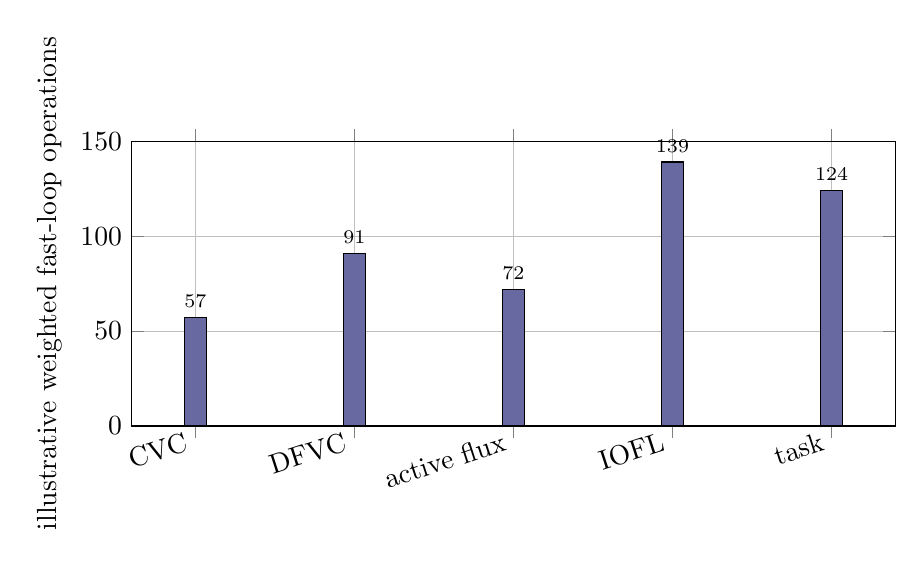
\begin{tikzpicture}
\begin{axis}[
 ybar,bar width=8pt,width=.93\textwidth,height=5.2cm,
 ylabel={illustrative weighted fast-loop operations},
 symbolic x coords={CVC,DFVC,active flux,IOFL,task},
 xtick=data,x tick label style={rotate=18,anchor=east},
 ymin=0,ymax=150,grid=major,
 nodes near coords,nodes near coords style={font=\scriptsize},
]
\addplot[fill=MidnightBlue!65] coordinates
 {(CVC,57) (DFVC,91) (active flux,72) (IOFL,139) (task,124)};
\end{axis}
\end{tikzpicture}
\caption{Weighted summary of the explicit count model
\((1\times\{\mathrm{mult,add,LUT}\},4\times\mathrm{div},
6\times\mathrm{sqrt},12\times\mathrm{CORDIC})\). Observer and matrix-solve
states are reported separately in the table and not hidden in these bars.}
\label{fig:operation-counts}
\end{figure}
